% Editable native composition from verified original IDE photographs.
\par
\begin{figure}[htbp]
\centering
\sbox0{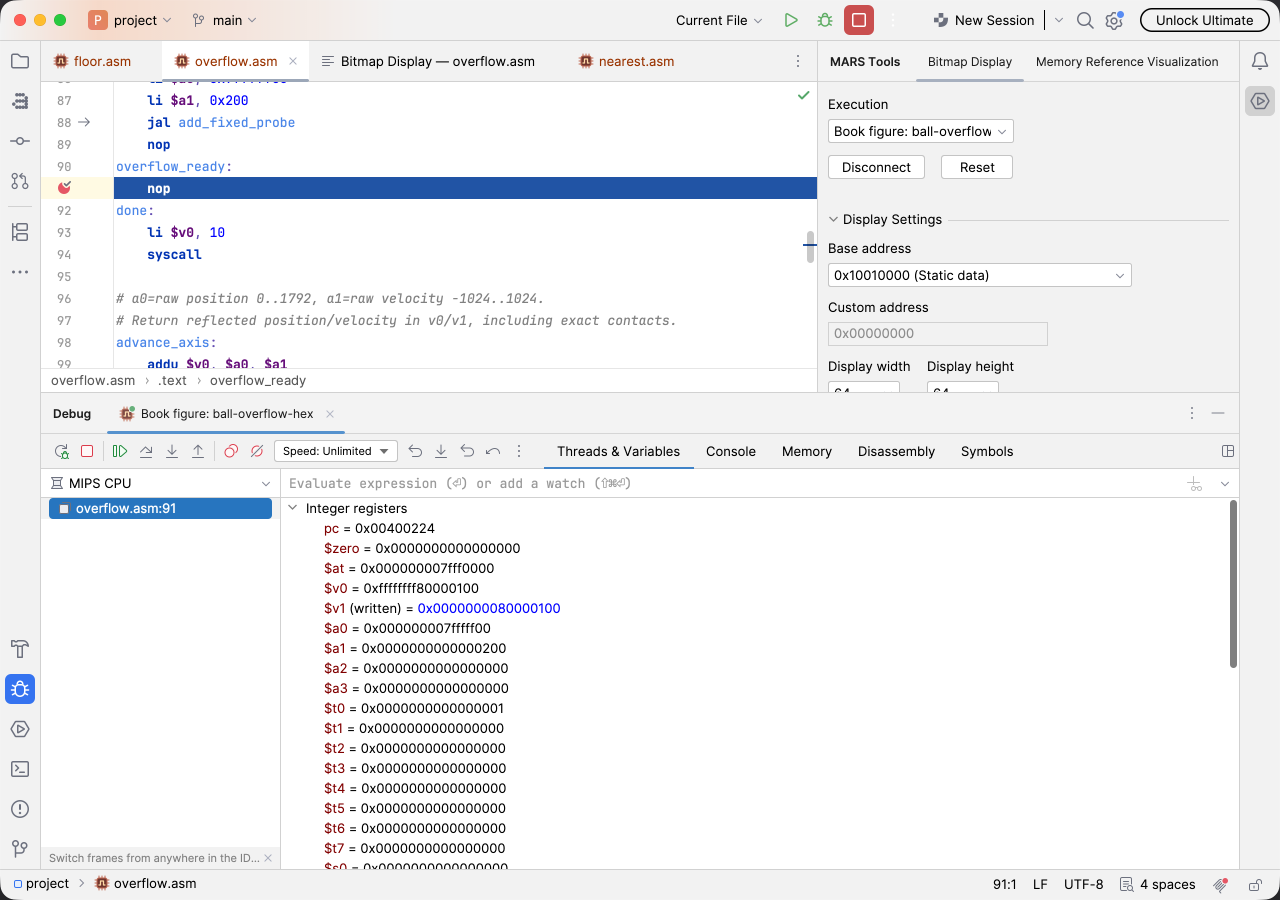
\includegraphics[artifact]{packages/012-fixed-point-ball/captures/f04-overflow/hex.png}}
\sbox2{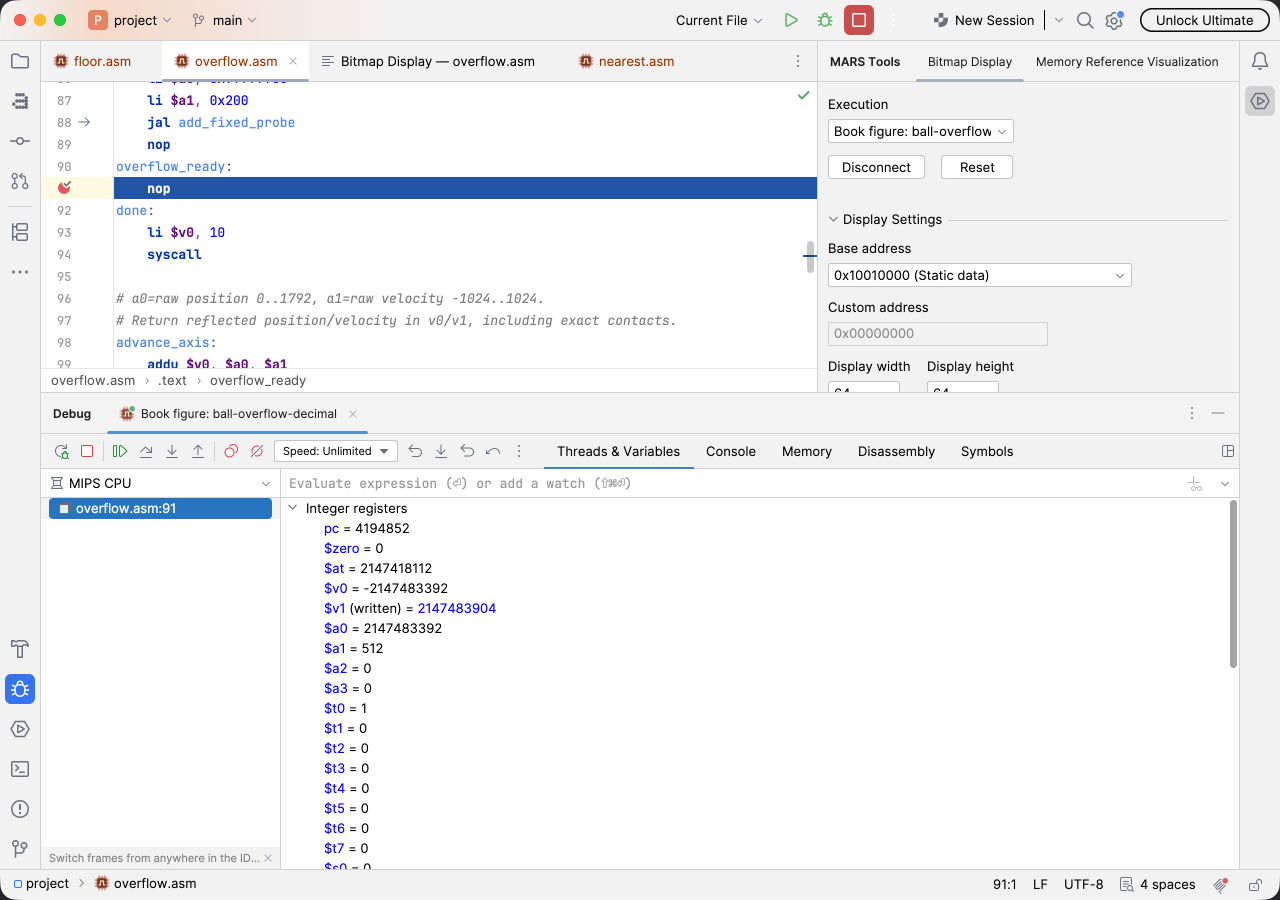
\includegraphics[artifact]{packages/012-fixed-point-ball/captures/f04-overflow/decimal.png}}
\edef\MARSballoverflowsourceLeft{\the\dimexpr0.036718750\wd0\relax}
\edef\MARSballoverflowsourceBottom{\the\dimexpr0.774444444\ht0\relax}
\edef\MARSballoverflowsourceRight{\the\dimexpr0.713281250\wd0\relax}
\edef\MARSballoverflowsourceTop{\the\dimexpr0.147777778\ht0\relax}
\edef\MARSballoverflowhexLeft{\the\dimexpr0.246093750\wd0\relax}
\edef\MARSballoverflowhexBottom{\the\dimexpr0.308888889\ht0\relax}
\edef\MARSballoverflowhexRight{\the\dimexpr0.556250000\wd0\relax}
\edef\MARSballoverflowhexTop{\the\dimexpr0.637777778\ht0\relax}
\edef\MARSballoverflowdecimalLeft{\the\dimexpr0.246093750\wd2\relax}
\edef\MARSballoverflowdecimalBottom{\the\dimexpr0.308888889\ht2\relax}
\edef\MARSballoverflowdecimalRight{\the\dimexpr0.606250000\wd2\relax}
\edef\MARSballoverflowdecimalTop{\the\dimexpr0.637777778\ht2\relax}
\begin{tikzpicture}[alt={Three annotated details from the same overflow experiment replayed in two Debug launches. The next instruction is the overflow ready marker before exit reuses v0. Hexadecimal v0 is ffffffff80000100 and v1 is 0000000080000100. The native decimal view shows minus 2147483392 and positive 2147483904 respectively. Ordinary ball state is never initialized on this path.}]
\node[anchor=north west,inner sep=0,font=\small\bfseries] (source-title) at (6mm,0) {Next instruction};
\node[anchor=north west,inner sep=0] (source) at ([yshift=-1mm]source-title.south west) {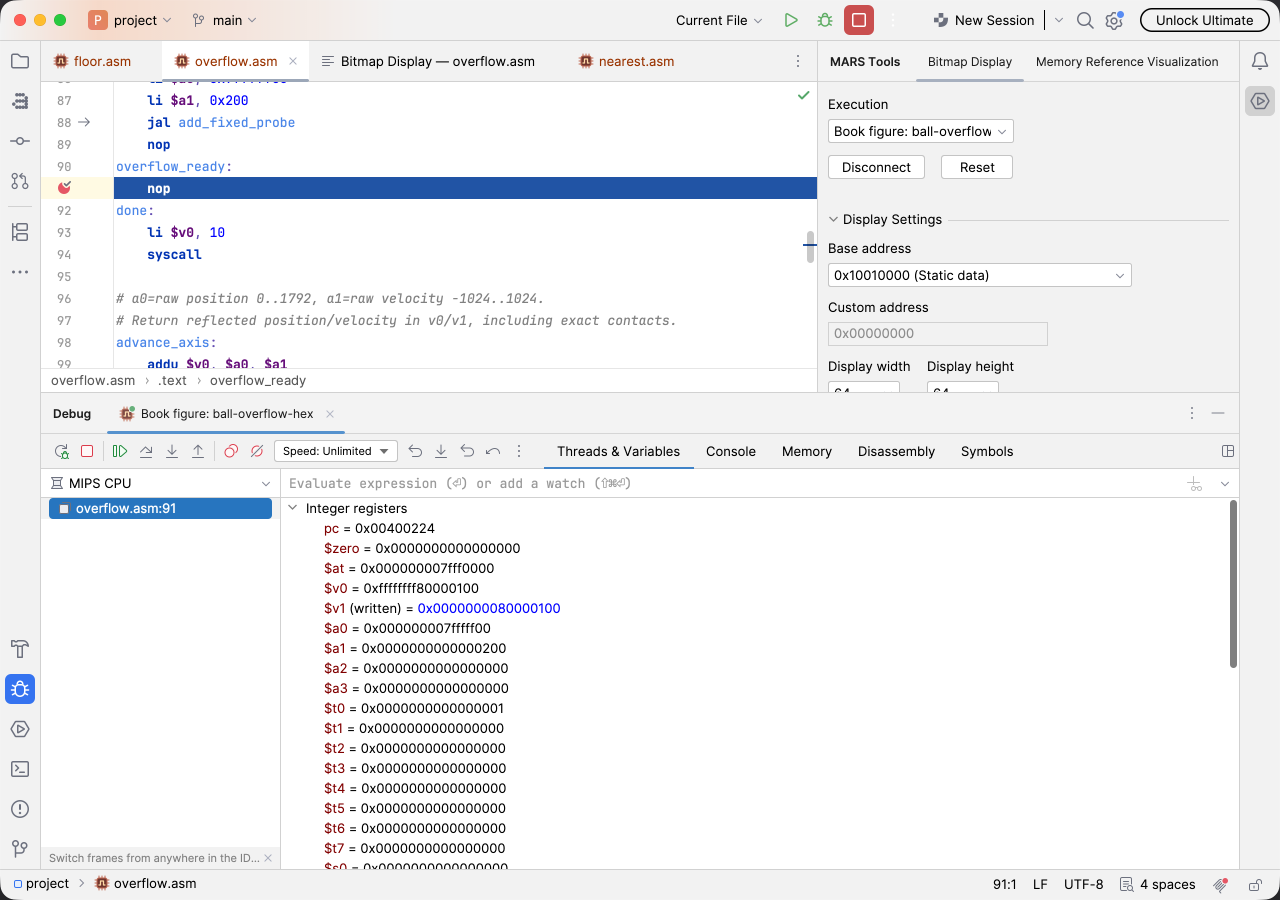
\includegraphics[width=0.58\linewidth,artifact,trim={\MARSballoverflowsourceLeft{} \MARSballoverflowsourceBottom{} \MARSballoverflowsourceRight{} \MARSballoverflowsourceTop{}},clip]{packages/012-fixed-point-ball/captures/f04-overflow/hex.png}};
\begin{scope}[shift={(source.south west)},x={($(source.south east)-(source.south west)$)},y={($(source.north west)-(source.south west)$)}]
\draw[black,line width=0.7pt] (0.215625000,0.057142857) rectangle (0.384375000,0.371428571);
\node[draw=black,fill=white,circle,inner sep=1.5pt,font=\footnotesize] at ($(0.215625000,0.371428571)+(-3mm,0)$) {1};
\end{scope}
\node[anchor=north west,inner sep=0,font=\small\bfseries] (hex-title) at ([yshift=-3mm]source.south west) {Native hexadecimal register view};
\node[anchor=north west,inner sep=0] (hex) at ([yshift=-1mm]hex-title.south west) {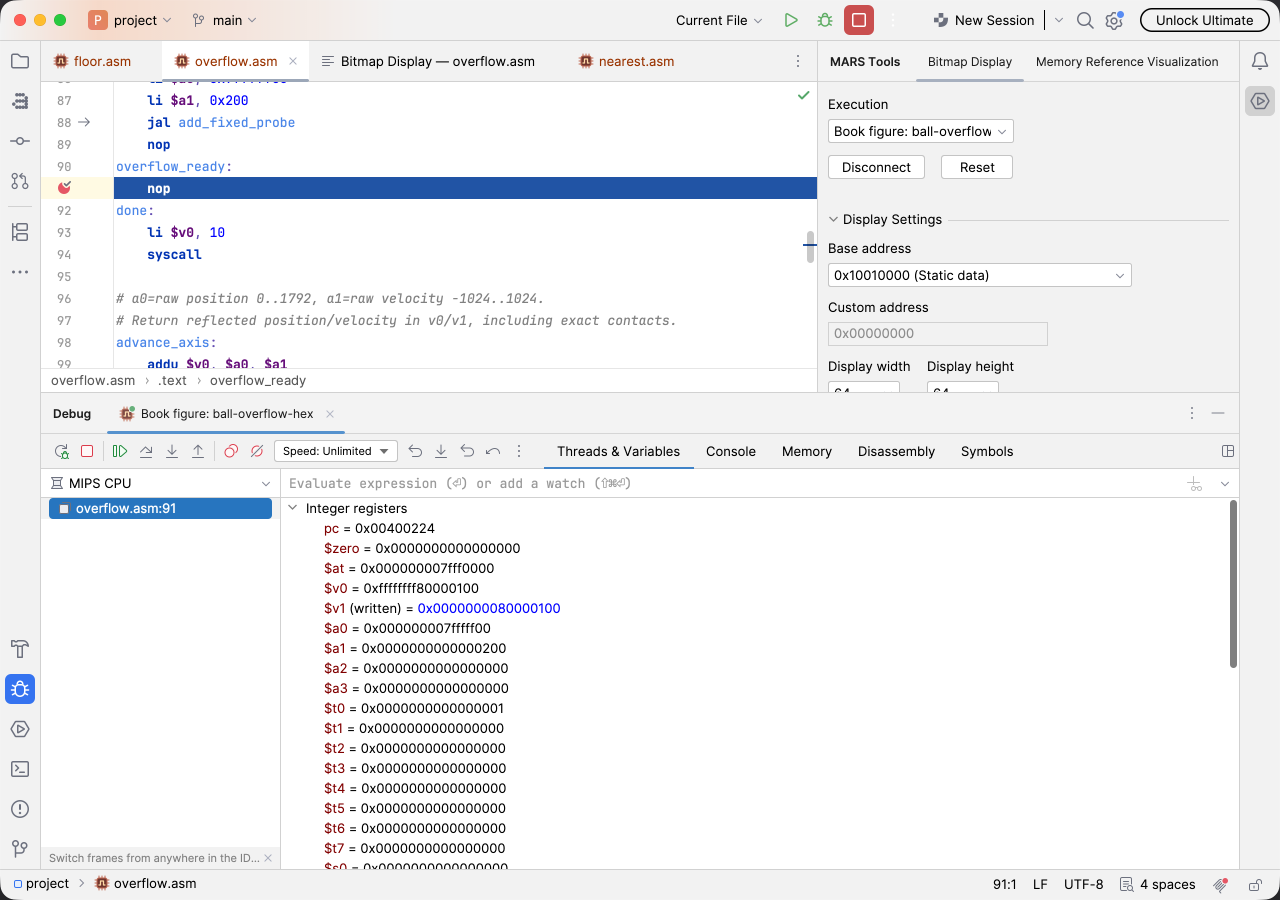
\includegraphics[width=0.48\linewidth,artifact,trim={\MARSballoverflowhexLeft{} \MARSballoverflowhexBottom{} \MARSballoverflowhexRight{} \MARSballoverflowhexTop{}},clip]{packages/012-fixed-point-ball/captures/f04-overflow/hex.png}};
\begin{scope}[shift={(hex.south west)},x={($(hex.south east)-(hex.south west)$)},y={($(hex.north west)-(hex.south west)$)}]
\draw[black,line width=0.7pt] (0.023715415,0.083333333) rectangle (0.976284585,0.916666667);
\node[draw=black,fill=white,circle,inner sep=1.5pt,font=\footnotesize] at ($(0.023715415,0.916666667)+(-3mm,0)$) {2};
\end{scope}
\node[anchor=north west,inner sep=0,font=\small\bfseries] (decimal-title) at ([yshift=-3mm]hex.south west) {Native signed-decimal register view};
\node[anchor=north west,inner sep=0] (decimal) at ([yshift=-1mm]decimal-title.south west) {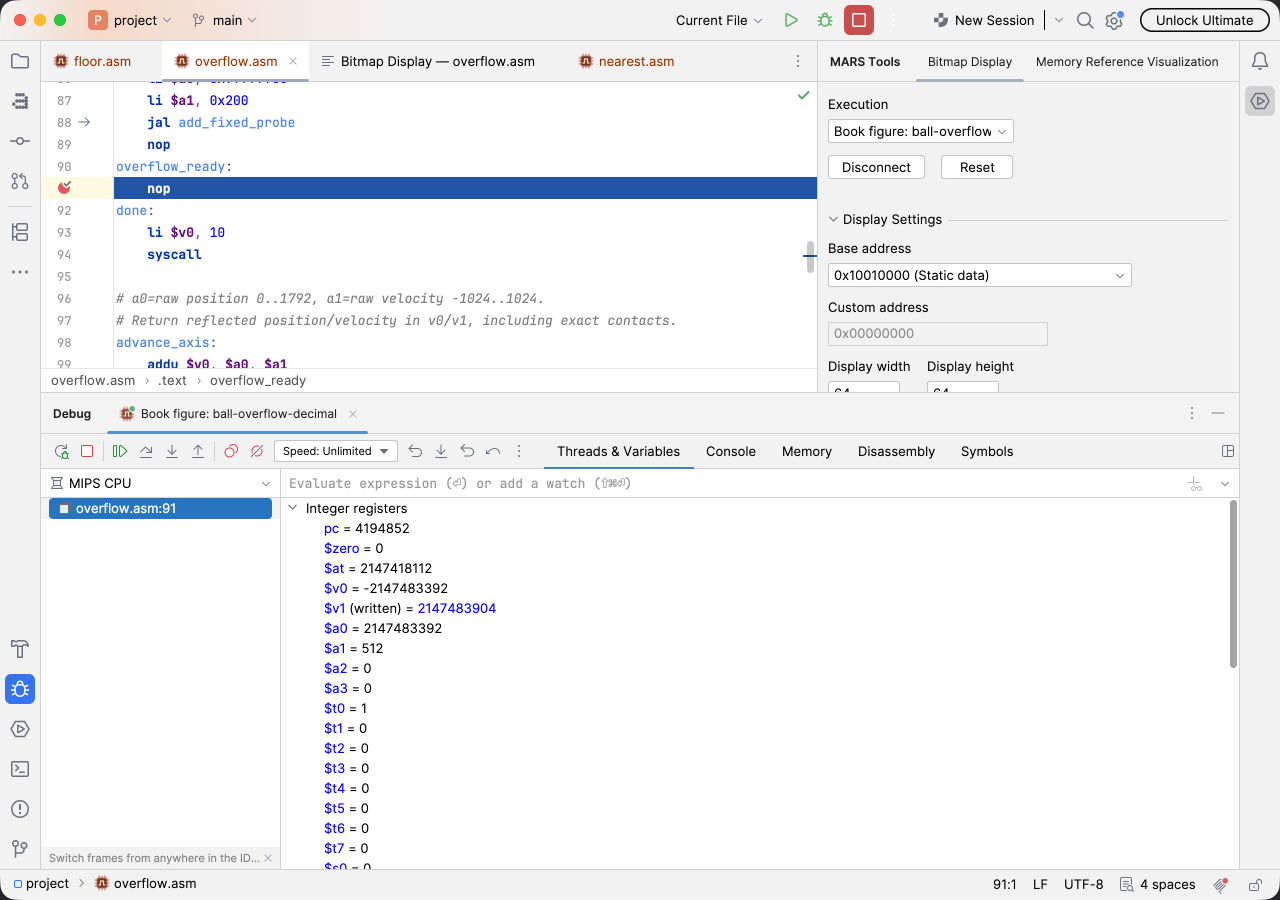
\includegraphics[width=0.48\linewidth,artifact,trim={\MARSballoverflowdecimalLeft{} \MARSballoverflowdecimalBottom{} \MARSballoverflowdecimalRight{} \MARSballoverflowdecimalTop{}},clip]{packages/012-fixed-point-ball/captures/f04-overflow/decimal.png}};
\begin{scope}[shift={(decimal.south west)},x={($(decimal.south east)-(decimal.south west)$)},y={($(decimal.north west)-(decimal.south west)$)}]
\draw[black,line width=0.7pt] (0.031746032,0.083333333) rectangle (0.968253968,0.916666667);
\node[draw=black,fill=white,circle,inner sep=1.5pt,font=\footnotesize] at ($(0.031746032,0.916666667)+(-3mm,0)$) {3};
\end{scope}
\end{tikzpicture}
\par\smallskip
\begin{minipage}{\linewidth}
\small
\begin{enumerate}
\setlength{\itemsep}{2pt}
\setlength{\parsep}{0pt}
\item Both launches use \texttt{DEMO = 1} and stop before the \texttt{overflow\_ready} marker. This path branches before animation initialization. Inspect here: normal exit will replace \texttt{\$v0} with service number 10. The launches differ only in the native register display base.
\item \texttt{addu} retains the low 32-bit result \texttt{0x80000100} and sign-extends it into \texttt{\$v0}, producing upper bits \texttt{ffffffff}. \texttt{daddu} computes the exact wider sum in \texttt{\$v1}, whose upper bits are zero. Matching low words therefore do not imply matching signed 64-bit values. The native \texttt{(written)} suffix identifies a recently written register; it is not part of the number.
\item The native decimal view shows \texttt{\$v0 = -2147483392} and \texttt{\$v1 = 2147483904}. The exact raw sum is $2147483392+512=2147483904$; with eight fractional bits it represents 8388609. Word wrapping instead represents $-8388607$. The binary-point convention does not prevent integer overflow. These operands belong to the separate numeric experiment, outside the bounded ball-motion domain.
\end{enumerate}
\end{minipage}
\caption{Native hexadecimal and signed-decimal views distinguish the wrapped word from the exact wider sum.}
\label{capture:012-fixed-point-ball-f04-overflow}
\label{ball-f04-overflow}
\end{figure}
\par
